\subsection{L1L2}

The following section describes the data set where one track misses Layer 1 of the SVT and its track projection back to Layer 1 is within 2.5~mm of the beam such that the track does not extrapolate to the active region of the silicon.

\subsubsection{Cuts}

The cuts applied to the L1L2 dataset with the first layer of the SVT at 1.5~mm is shown in Table~\ref{l1l2_cuts_1p5}.

\begin{table}[H]
\caption{Cuts applied to the L1L2 datasets with the SVT at 1.5~mm.}
\label{l1l2_cuts_1p5}
\centering
\begin{tabular}{lllllll}
\toprule
%\multicolumn{2}{c}{Name} \\
%\cmidrule(r){1-2}
Cut type & Cut & Cut Value &  $\%$killed &  $\%$killed core & $\%$killed tails\\
\midrule
track & Fit quality & track $\chi^{2}<30$ & 23 & 11 & 47 \\
track & Max track momentum &  $P_{trk}<75\%E_{beam}$ & 8 & 7 & 12 \\
track & Isolation &   & 4 & 2 & 10 \\
vertex & beamspot constraint & bsc$\chi^{2}<10$  & 29 & 20 & 62 \\
vertex & beamspot - unconstrained & bsc$\chi^{2}$-unc$\chi^2<5$  & 12 & 11 & 22 \\
vertex & maximum $P_{sum}$ &  $<115\%E_{beam}$ & 0 & 0 & 0 \\
ecal & Ecal SVT matching & $\chi^2<10$  & 5 & 5 & 7 \\
ecal & track Ecal timing & $<4$ns  & 5 & 5 & 5 \\
ecal & 2 cluster time diff & $<2$ns  & 6 & 5 & 9 \\
physics & momentum asymmetry & $<0.4$  & 14 & 13 & 16 \\
physics & e+ track d0 & $<1.5$mm  & 6 & 5 & 16 \\
event & max shared hits amongst tracks & $<5$ shared hits  & 6 & 6 & 6 \\
track & cuts on kink tails & $\phi$ and $\lambda$ kink tails & 22 & 8 & 74 \\
\bottomrule
\end{tabular}
\end{table}

The cuts applied to the L1L2 dataset may require a similar optimization to eliminate backgrounds as that required of the dataset for the 0.5~mm. Namely, that, it may be necessary to separate the dataset for events where the positron versus the electron is the first to leave a hit in Layer 1. For the moment, the same cuts are used as the 1.5~mm dataset has generally lower backgrounds than that seen in the 0.5~mm dataset.

\subsubsection{Vertex reconstruction efficiency, $\epsilon_{vtx}$}

The vertex reconstruction efficiency is fit for each simulated heavy photon mass using a Crystal Ball function as described in Equation~\eqref{eq:cbfunction}. The parameters of the fit can described as a function of mass as shown in Equation~\eqref{eq:parsEpsVtxL1L2_1p5}.

\begin{eqnarray*}
\label{eq:parsEpsVtxL1L2_1p5}
z_{mean} & = & -64.13+3.97m-0.033m^2 \\
\sigma & = & 8.166+0.062m \\
N & = & 0.12+0.0153m-0.00023m^2 \\
\end{eqnarray*}

 Having fully characterized the vertex reconstruction efficiency in terms of mass and z position for the L1L2 dataset, one can observe the integral value from Equation~\eqref{eq:signal} as a function zCut and mass as shown in Figure~\ref{fig:integral_L1L2_1p5} where zMax is 80~mm due to acceptance.

\begin{figure}[H]
  \centering
     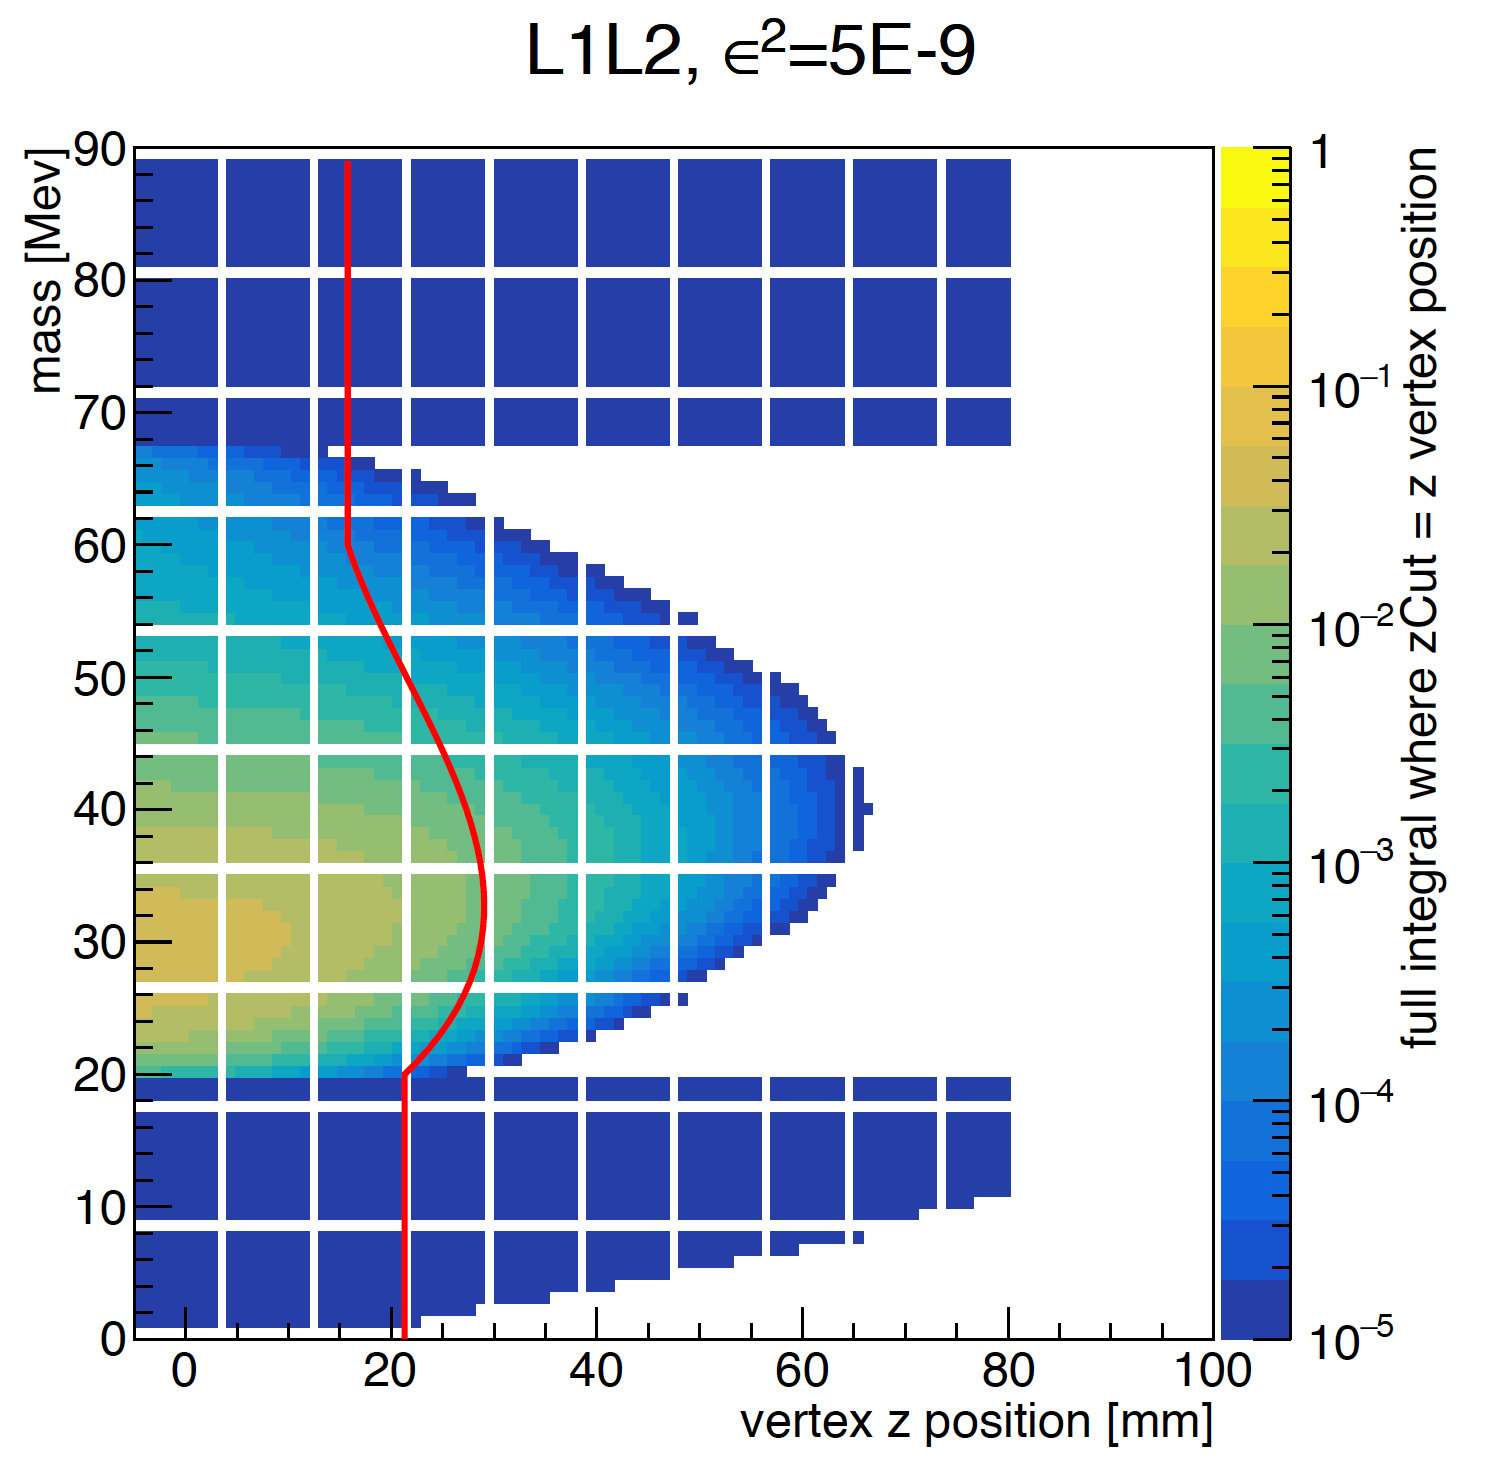
\includegraphics[width=0.8\textwidth]{plots/L1L2_eff1p5_zm.png}
  \caption{This plot, for fixed coupling $\epsilon^2$, shows the fraction of signal events that will be measured as a function of the integral using the vertex position along the x-axis as the $zCut$. The red line indicates the position of the $zCut$ as found for the 10$\%$ sample.}
  \label{fig:integral_L1L2_1p5}
\end{figure} 

The red line shown in Figure~\ref{fig:integral_L1L2_1p5} shows where the zCut value lies that was obtained for the L1L2 dataset. The fraction of events is significantly less by an approximate order of magnitude when compared to the L1L1 dataset, but the zCut seems well optimized to maintain reach.

\subsubsection{Accidentals}

No accidental high z background events were identified when selecting the out of time events using the methods discussed previously. 

\subsubsection{Projected reach}

The final vertex distribution as a function of mass is shown in Figure~\ref{fig:zVm_L1L2_1p5}. 
\begin{figure}[H]
  \centering
     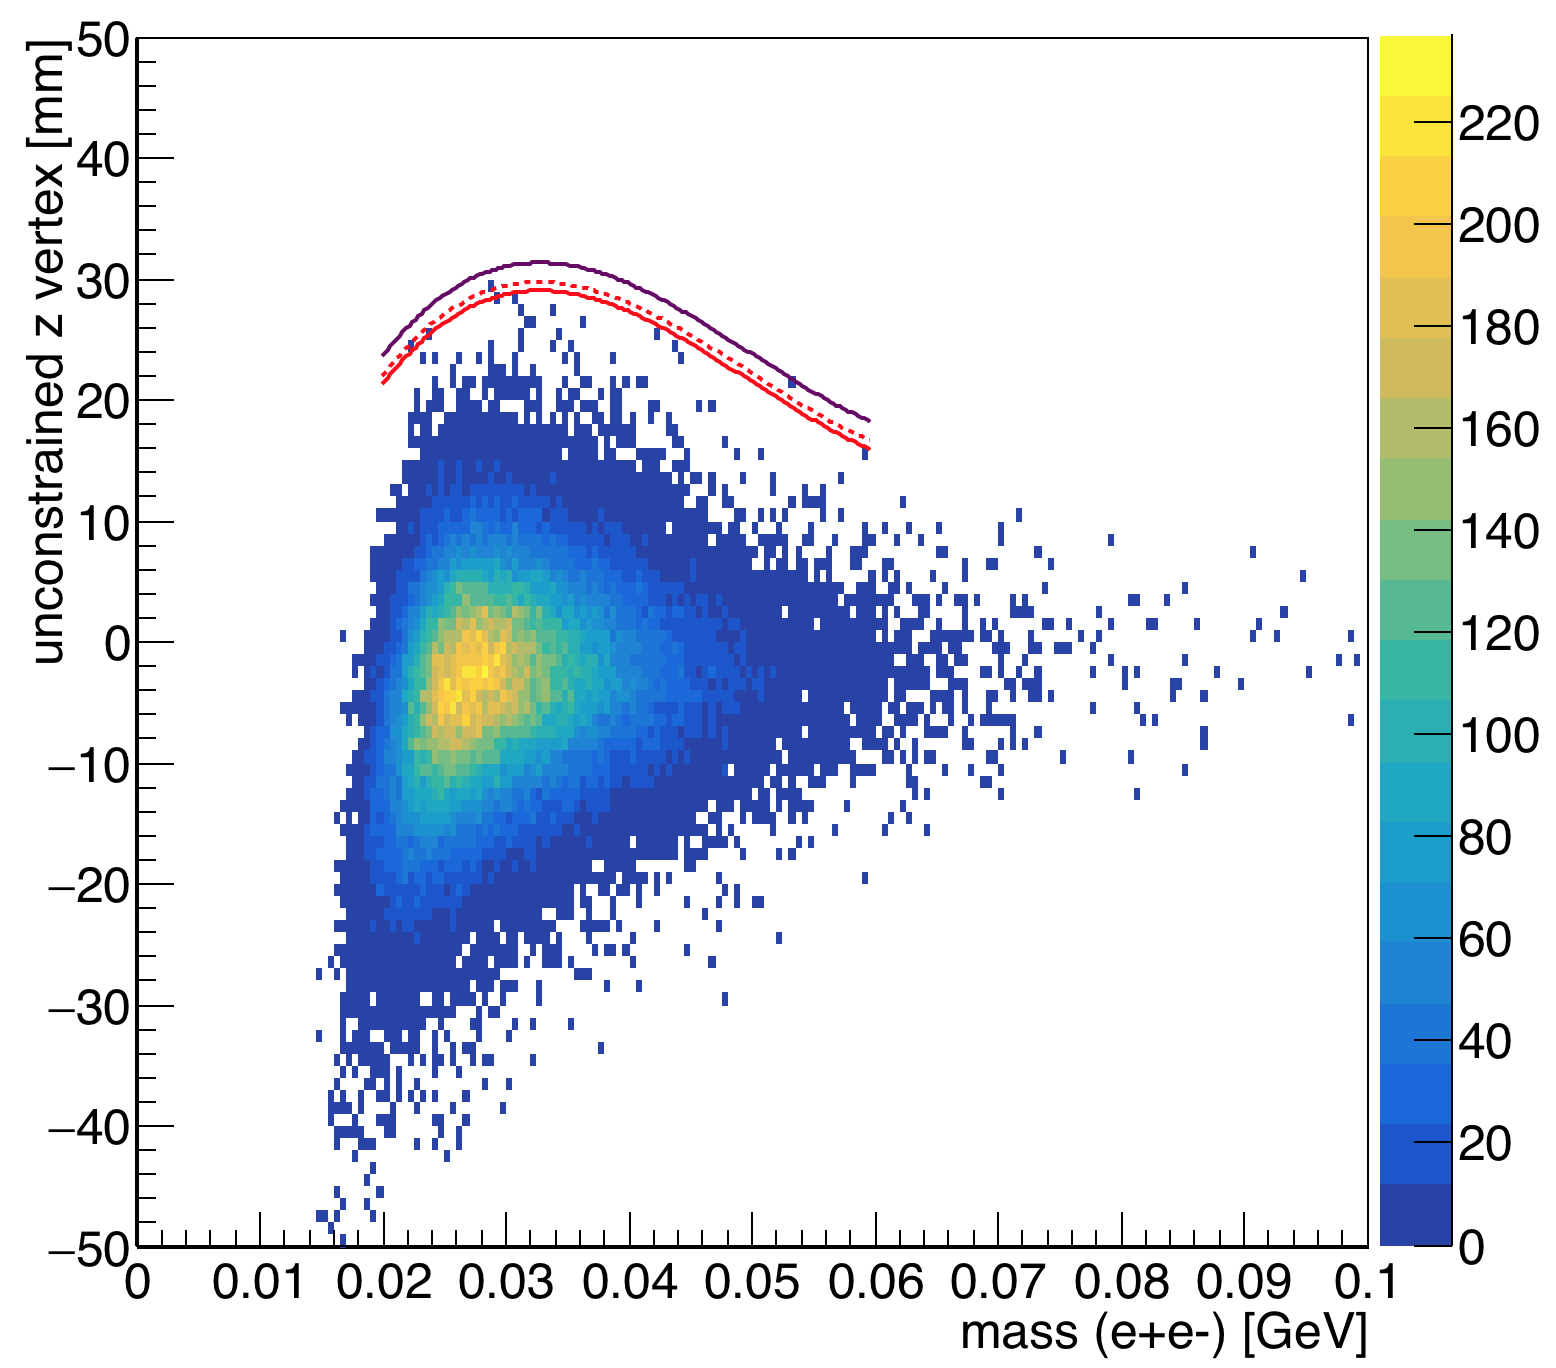
\includegraphics[width=0.8\textwidth]{plots/zVm_L1L2_1p5.png}
  \caption{Reconstructed z vertex as a function of mass for the L1L2 dataset with the first layer of the SVT at 1.5~mm from the beam. The solid red line indicates the zCut found for 10$\%$ of the data (unblinded), and the dashed red line indicates the limit at which events have a quantile greater than 0.5 with respect to the predicted background model. The purple line shows where the projected zCut will be for the full dataset after unblinding.}
  \label{fig:zVm_L1L2_1p5}
\end{figure} 

Using the zCut shown in Figure~\ref{fig:zVm_L1L2_1p5}, we can calculate the expected signal reach for the L1L2 dataset. The reach is shown in Figure~\ref{fig:reach1p5_l1l2}.

\begin{figure}[H]
  \centering
     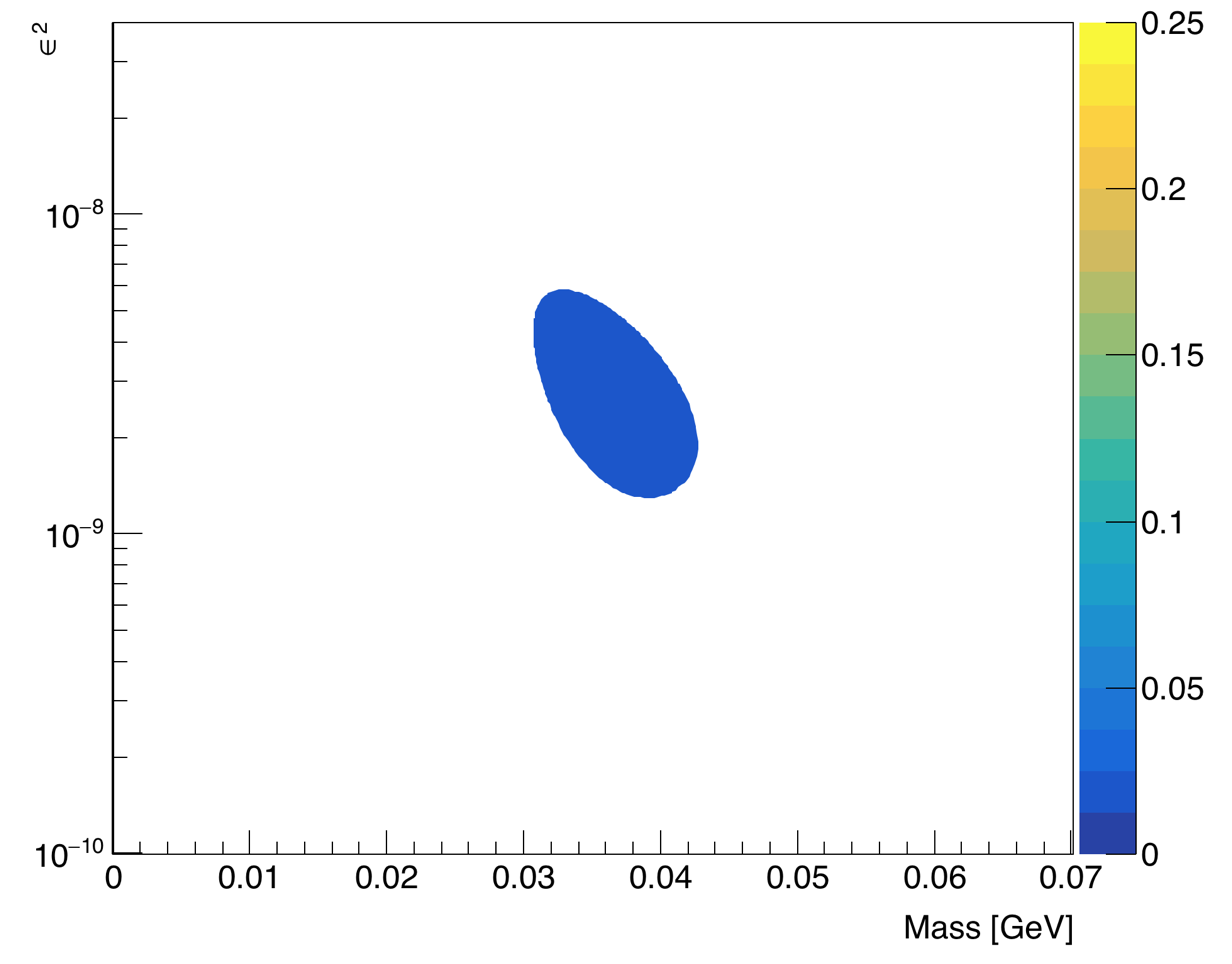
\includegraphics[width=0.8\textwidth]{plots/reachL1L2_1p5.png}
  \caption{The expected signal yield for the full 100$\%$ dataset with the L1L2 1.5~mm data.}
  \label{fig:reach1p5_l1l2}
\end{figure} 

The L1L2 dataset favors higher masses than the L1L1 dataset and has the highest yield in the relatively central region of the coupling reach for the 2015 run. 
